\sectioncounter{21}

\section{余弦定理与解三角形}

设 $\triangle ABC$ 中, 角 $A$, $B$, $C$ 的对边分别为 $a$, $b$, $c$, 
则由直角坐标系中的距离公式或向量的内积运算可得余弦定理: 
\[a^2= b^2+ c^2- 2bc\cos A,\quad\cos A=\frac{b^2+c^2-a^2}{2bc}.\]
现用前一种方法推导. 如图 \ref{fig:2021-0312-2130} 所示, 
\mymarginpar{推导过程中无需假设 $A$ 为锐角, 即当 $A$ 为直角或钝角时, 推导过程仍有效.}
$C$ 的坐标 $(b\cos A,b\sin A)$ 由三角函数定义得到. 由 $BC=a$ 知 $BC^2= a^2$, 即
\[(c-b\cos A)^2+ (b\sin A)^2= a^2,\]
整理即得要证的公式. 

\begin{figure}[hb]
    \centering
    \includegraphics[scale=1.5]{2021-0312-2130-crop}
    \caption{}\label{fig:2021-0312-2130}
\end{figure}

还可以写出
\[b^2= a^2+ c^2- 2ac\cos B,\quad\cos C=\frac{a^2+b^2-c^2}{2ab},\]
即余弦定理共三组公式. 勾股定理可以视为余弦定理的特例 (如令 $C=\dfrac\pi2$, 可知 $c^2= a^2+b^2$). 在解三角形时, 一般题中已知等式里角多则先考虑用正弦定理, 边多则先考虑用余弦定理.

\lianxi
\begin{exercise}
    在 $\triangle ABC$ 中, 若 $a:b:c=2:3:4$, 求 $\cos C$ 的值.
\end{exercise}
\beginsolution
    设 $a=2k$, $b=3k$, $c=4k$, $k>0$, 则
    \mymarginpar{由连等式引入公因子 $k$, 可将各变量用 $k$ 表示.}
    \[\cos C= \dfrac{a^2+b^2-c^2}{2ab}= -\frac14.\]
\endsolution

\begin{exercise}
    在 $\triangle ABC$ 中, 若 $a=\sqrt2$, $b=2$, $c=1+\sqrt3$, 求 $A$ 的大小.
\end{exercise}
\beginsolution
    由余弦定理得 $\cos A= \dfrac{\sqrt3}2$, 所以 $A=\dfrac\pi6$.
\endsolution

\begin{exercise}
    在 $\triangle ABC$ 中, $(a+b+c)(b+c-a)=3bc$, 求 $A$ 的大小.
\end{exercise}
\beginsolution
    已知式改写为
    \[ [(b+c)+ a][(b+c)-a]= 3bc,\]
    展开后整理得 $b^2+c^2-a^2= bc$. 由余弦定理, $\cos A= \dfrac12$, $A=\dfrac\pi3$.
\endsolution

\begin{exercise}
    若 $\triangle ABC$ 中 $c=2a\cos B$, 确定 $\triangle ABC$ 的形状.
\end{exercise}
\beginsolution
    方法一: 已知式化为 $c=2a\cdot \dfrac{a^2+c^2- b^2}{2ac}$, 整理得 $a^2= b^2$, 即 $a=b$. 所以 $\triangle ABC$ 为等腰三角形.

    方法二: 由正弦定理, $\sin C= 2\sin A\cos B$, 而
    \[\sin C= \sin(A+B)= \sin A\cos B+ \cos A\sin B,\]
    联立可得 $\sin A\cos B- \cos A\sin B= 0$, 
    \mymarginpar{此处也可得到 $\tan A=\tan B$, 故 $A=B$.}
    即 $\sin(A-B)= 0$. 所以 $A=B$, 结论同上.
\endsolution

\begin{exercise}
    在 $\triangle ABC$ 中, 若 $a=4$, $b=5$, $c=6$, 求 $\triangle ABC$ 的面积.
\end{exercise}
\beginsolution
    由余弦定理, $\cos C= \dfrac18$, 
    \mymarginpar{一般地, 对 $\triangle ABC$, 设 $p= \dfrac12(a+b+c)$ (称其为半周长), 则
    \[S_{\triangle ABC}= \sqrt{p(p-a)(p-b)(p-c)}.\]
    上式也称为海伦 (Heron) 公式.}
    所以 $\sin C= \dfrac{\sqrt{63}}8$,
    \[S_{\triangle ABC}= \frac12 ab\sin C= \frac{5\sqrt{63}}{4}.\]
\endsolution

\subsection{要点导学\quad 各个击破}
\subsubsection{余弦定理的简单应用}
\begin{example}
    在 $\triangle ABC$ 中 $a^2 =b^2+c^2+ \sqrt3 bc$, 求角 $A$ 的大小.
\end{example}
\beginsolution
    易知 $\cos A= -\dfrac{\sqrt3}2$, 所以 $A= \dfrac{5\pi}6$.
\endsolution

\begin{example}
    $\triangle ABC$ 中 $B=\dfrac{2\pi}3$, $b=\sqrt{13}$, $a+c=4$, 
    求 $\triangle ABC$ 的面积.
\end{example}
\beginsolution
    因为 $b^2= a^2+c^2- 2ac\cos B$, 所以 
    \[13= a^2+c^2+ac,\quad\text{即}\quad (a+c)^2= 13+ac.\]
    将 $a+c=4$ 代入知 $ac=3$, 故
    \mymarginpar{此题无需算出 $a$, $c$ 的具体值.}
    \[S_{\triangle ABC}= \frac12 ac\sin B= \frac{3\sqrt{3}}{4}.\]
\endsolution

\lianxi
\begin{exercise}
    在 $\triangle ABC$ 中 $(a+b+c)(a+b-c)= ab$, 求角 $C$ 的大小.
\end{exercise}
\beginsolution
    已知式整理为 $a^2+b^2- c^2= -ab$, 所以 $\cos C= -\dfrac12$, $C= \dfrac{2\pi}3$.
\endsolution

\begin{exercise}
    在 $\triangle ABC$ 中 $(a^2 +c^2 -b^2 )\tan B=\sqrt3 ac$, 求角 $B$ 的大小.
\end{exercise}
\beginsolution
    已知式化为
    \[2ac\cos B\tan B= \sqrt3 ac,\quad\text{即}\quad
        \sin B= \dfrac{\sqrt3}2,\]
    所以 $B= \dfrac\pi3$ 或 $\dfrac{2\pi}3$.
\endsolution

\subsubsection{余弦定理的综合应用}
\begin{example}
    已知 $\triangle ABC$ 的内角 $A$, $B$, $C$ 所对的边分别为 $a$, $b$, $c$.
    
    (1) 若 $a$, $b$, $c$ 成等差数列, 求证: $\sin A+\sin C=2\sin (A+C)$;
    
    (2) 若 $a$, $b$, $c$ 成等比数列, 求 $\cos B$ 的最小值.
\end{example}
\beginsolution
    (1) 由题意, $2b= a+c$, 即
    \[2\sin B= \sin A+ \sin C.\]
    由 $A+B+C= \pi$ 知 $\sin B= \sin(A+C)$, 代入知结论成立.

    (2) 由已知,
    \[b^2= ac= a^2+c^2- 2ac\cos B,\]
    则 $\cos B= \dfrac{a^2+c^2- ac}{2ac}$. 
    \mymarginpar{由 (2) 可得, $B\leqslant \dfrac\pi3$.}
    因为 $a^2+c^2\geqslant 2ac$, 所以 $\cos B\geqslant \dfrac12$.
\endsolution

\lianxi
\begin{exercise}[s]
    已知 $\triangle ABC$ 的周长为 $4(\sqrt2+1)$, 且 $\sin B+\sin C=\sqrt2\sin A$.
    
    (1) 求 $a$ 的值;\qquad
    (2) 若 $S_{\triangle ABC}= 3\sin A$, 求 $\cos A$ 的值.
\end{exercise}
\beginsolution
    (1) 由题意,
    \[\left\{\!\!\begin{array}{l}
        b+c= \sqrt2 a,\\
        a+b+c= 4(\sqrt2+ 1),
    \end{array}\right.\ \text{解得}\quad a=4.\]

    (2) 由面积定理, $\dfrac12 bc\sin A= 3\sin A$, 即 $bc= 6$. 而 $b+c= 4\sqrt2$, 所以
    \[b^2+c^2= (b+c)^2- 2bc= 20,\]
    继而可知 $\cos A= \dfrac13$.
\endsolution

\subsubsection{正弦、余弦定理的几何应用}

\begin{example}
    如图~\ref{fig-180801-1920}, 在平面四边形 $ABCD$ 中, $AD=1$, $CD=2$, $AC=\sqrt7$.
    
    (1) 求 $\cos\angle CAD$ 的值;
    
    (2) 若 $\cos\angle BAD=-\dfrac{\sqrt7}{14}$, $\sin \angle CBA=\dfrac{\sqrt{21}}6$, 求 $BC$ 的长.
\end{example}
\beginsolution
    (1) 在 $\triangle ACD$ 中用余弦定理, $\cos\angle CAD= \dfrac{2\sqrt7}7$.

    (2) 因为 $\sin\angle BAD= \dfrac{3\sqrt3}{2\sqrt7}$, $\sin\angle CAD= \dfrac{\sqrt3}{\sqrt7}$, 所以
    \[\sin\angle BAC= \sin(\angle BAD- \angle CAD)
        = \dfrac{\sqrt3}2.\]
    在 $\triangle ABC$ 中用正弦定理, 
    \[\frac{BC}{\sin\angle BAC}= \dfrac{AC}{\sin\angle CBA},\quad
    \text{即}\quad BC= 3.\]
\endsolution

\begin{figure}[htb]
\small
\centering
\begin{minipage}[b]{0.45\linewidth}
    \centering
    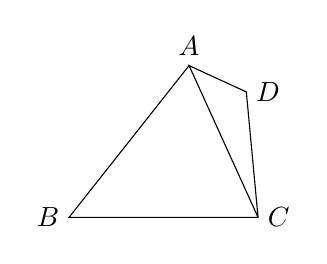
\begin{tikzpicture}[scale=0.8]
      \draw (1.905,2.409) coordinate (A) node[above] {$A$};
      \draw (0,0) coordinate (B) node[left] {$B$};
      \draw (3,0) coordinate (C) node[right] {$C$};
      \draw (2.814,1.991) coordinate (D) node[right] {$D$};
      \draw (A)--(B)--(C)--(A)--(D)--(C) (C)--(A);
    \end{tikzpicture}
\caption{}\label{fig-180801-1920}
\end{minipage}
\hskip 0.5cm%
\begin{minipage}[b]{0.45\linewidth}
    \centering
    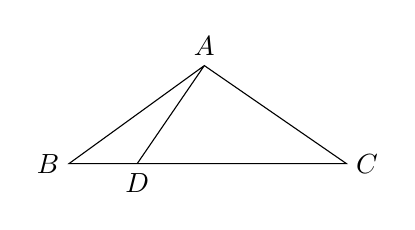
\begin{tikzpicture}[scale=0.5]
      \draw (3.436,2.489) coordinate (A) node[above] {$A$};
      \draw (0,0) coordinate (B) node[left] {$B$};
      \draw (7.044,0) coordinate (C) node[right] {$C$};
      \draw (1.732,0) coordinate (D) node[below] {$D$};
      \draw (A)--(B)--(C)--(A)--(D);
    \end{tikzpicture}
\caption{}\label{fig-180801-1935}
\end{minipage}
\end{figure}
    
\lianxi
\begin{exercise}[s]
    如图~\ref{fig-180801-1935}, 在 $\triangle ABC$ 中, 点 $D$ 在 $BC$ 边上, $AD\perp AC$, $\sin \angle BAC= \dfrac{2\sqrt2}3$, $AB=3\sqrt2$, $AD=3$, 求 $BD$ 的长.
\end{exercise}
\beginsolution
    由题意, $\sin(\angle BAD+ 90^\circ)= \dfrac{2\sqrt3}3$, 即 $\cos\angle BAD= \dfrac{2\sqrt3}3$, 所以
    \[BD^2= AB^2+AD^2- 2AB\cdot AD\cos\angle BAD= 3,\]
    解得 $BD=\sqrt3$.
\endsolution

\subsubsection{课堂评价}
\begin{exercise}
    在 $\triangle ABC$ 中, 若 $\sin A:\sin B:\sin C=7:8:13$, 求 $\cos C$ 的值.
\end{exercise}
\beginsolution
    已知式化为 $a:b:c= 7:8:13$, 所以设 $a=7k$, $b=8k$, $c=13k$, $k>0$, 则 $\cos C= -\dfrac12$, 即 $C= \dfrac{2\pi}3$.
\endsolution

\begin{exercise}
    在 $\triangle ABC$ 中 $b-c=\dfrac14 a$, $2\sin B=3\sin C$, 求 $\cos A$ 的值.
\end{exercise}
\beginsolution
    由已知, $2b=3c$, 与 $b-c=\dfrac14 a$ 联立知, 
    \mymarginpar{将变量的倍数关系化为整数比例式, 可简化计算.}
    $b=\dfrac{3a}4$, $c=\dfrac{a}2$, 所以 $a:b:c= 4:3:2$, 而 $\cos A= -\dfrac14$.
\endsolution

\begin{exercise}
    在 $\triangle ABC$ 中 $(a+b)(\sin A-\sin B)=(c-b)\sin C$, 求角 $A$ 的大小.
\end{exercise}
\beginsolution
    已知式化为
    \[(a+b)(a-b)= (c-b)c,\]
    即 $b^2+c^2- a^2= bc$, 所以 $\cos A= \dfrac12$, 而 $A= \dfrac\pi3$.
\endsolution

\begin{exercise}
    在 $\triangle ABC$ 中 $a^2-b^2 = \sqrt3bc$, $\sin C=2\sqrt3\sin B$, 求 $A$ 的值.
\end{exercise}
\beginsolution
    后一式化为 $c= 2\sqrt3b$, 代入前一式,
    \[a^2-b^2= 6b^2,\quad\text{即}\quad a= \sqrt7b,\]
    所以 $\cos A= \dfrac{\sqrt3}2$, 得 $A= \dfrac\pi6$.
\endsolution

\subsection{课后练习}
\begin{exercise}
    在 $\triangle ABC$ 中 $a=2$, $B= \dfrac\pi6$, $c=2\sqrt3$, 求 $b$ 的值.
\end{exercise}
\beginsolution
    $b^2= a^2+c^2- 2ac\cos B= 4$, 则 $b=2$.
\endsolution

\begin{exercise}
    在 $\triangle ABC$ 中 $c^2=(a-b)^2 +6$, $C=\dfrac\pi3$, 求 $\triangle ABC$ 的面积.
\end{exercise}
\beginsolution
    由已知式和余弦定理,
    \[\begin{aligned}
        c^2&= a^2+b^2- 2ab +6\\
        &= a^2+b^2- ab,
    \end{aligned}\]
    所以 $ab=6$, $S_{\triangle ABC}= \dfrac{3\sqrt3}2$.
\endsolution

\begin{exercise}
    在锐角三角形 $ABC$ 中 $23\cos^2 A+\cos2A=0$, $a=7$, $c=6$, 求 $b$ 的值.
\end{exercise}
\beginsolution
    将 $\cos 2A= 2\cos^2 A-1$ 代入第一式, 可解得 $|\cos A|= \dfrac15$. 由题意, $A< \dfrac\pi2$, 则
    \[\cos A= \frac15= \frac{b^2+c^2- a^2}{2bc},\]
    整理得 $(5b+13)(b-5)= 0$, 故 $b= 5$.
\endsolution

\begin{exercise}
    在 $\triangle ABC$ 中, $B=120^\circ$, $AC=7$, $AB=5$, 求 $\triangle ABC$ 的面积.
\end{exercise}
\beginsolution
    由余弦定理, 
    \[AC^2= AB^2+ BC^2- 2AB\cdot BC\cos B,\]
    解得 $BC= 3$, 所以
    \[S_{\triangle ABC}= \frac12 ac\sin B= \dfrac{15\sqrt3}4.\]
\endsolution

\begin{exercise}
    在 $\triangle ABC$ 中, 若 $BC=3$, $B=120^\circ$, 且 $\triangle ABC$ 的面积为 $\dfrac{15\sqrt3}4$, 求 $AB$, $AC$ 的长.
\end{exercise}
\beginsolution
    由已知, $a=3$, 代入余弦定理,
    \[\begin{aligned}
        b^2&= a^2+c^2- 2ac\cos B\\
        &= 9+c^2- 3c.
    \end{aligned}\]
    再由 $S_{\triangle ABC}= \dfrac12 ac\sin B= \dfrac{15\sqrt3}4$ 知 $ac=15$, 即 $c=5$. 所以再由余弦定理, $b=7$. 因此 $AB=5$, $AC=7$.

    \varexercise 若 $AC=3$, $B=120^\circ$, 且 $\triangle ABC$ 的面积为 $\dfrac{15\sqrt3}4$, 求 $AB$, $AC$ 的长.

    思路不变, 此时
    \[\left\{\!\!\begin{array}{l}
        49= a^2+c^2+ac,\\
        \frac12 ac\cdot \frac{\sqrt3}{2}= \dfrac{15\sqrt3}4,
    \end{array}\right.\ \text{即}\ 
    \left\{\!\!\begin{array}{l}
        a+c= 8,\\
        ac=15,
    \end{array}\right.\]
    解得 $a=3$, $c=5$ 或 $a=5$, $c=3$.
\endsolution

\begin{exercise}
    若 $\triangle ABC$ 的面积为 $42$, $\cos B=\dfrac45$, $a=10$,  
    求 $b+\dfrac{a}{\sin A}$ 的值.
\end{exercise}
\beginsolution
    由题意, $\sin B= \dfrac35$, 
    \mymarginpar{本题无需计算 $\sin A$.}
    且 $\dfrac12 ac\sin B= 42$, 所以 $c=14$. 因为
    \[b^2= a^2+c^2- 2ac\cos B= 72,\]
    所以 $b= 6\sqrt2$, 而
    \[\frac{a}{\sin A}= \frac{b}{\sin B}= 10\sqrt2,\]
    故 $b+\dfrac{a}{\sin A}= 16\sqrt2$.
\endsolution

\begin{exercise}
    如图 \ref{fig:2021-0314-1240}, 设正方形 $ABCD$ 的边长为 $a$. 延长 $BA$ 至点 $E$, 使 $AE=a$, 连接 $EC$, $ED$, 求 $\sin\angle CED$ 的值.
\end{exercise}
\beginsolution
    方法一: 由题意, 
    \mymarginpar{四种解法各有特点, 均为常见解法.}
    $CD=a$, $DE=\sqrt2 a$, $CE= \sqrt5 a$, 所以
    \[\cos\angle CED= \frac{EC^2+ED^2- CD^2}{2EC\cdot ED}
        = \frac3{\sqrt{10}},\]
    而 $\sin\angle CED= \dfrac1{\sqrt{10}}= \dfrac{\sqrt{10}}{10}$.

    方法二: 因为 $\tan\angle AED= 1$, $\tan\angle AEC= \dfrac12$, 所以
    \[\tan\angle CED= \tan(\angle AED- \angle AEC)= \frac13,\]
    而 $\sin\angle CED= \dfrac{\sqrt{10}}{10}$.

    方法三: 因为 $\cos\angle AED= \sin\angle AED= \dfrac1{\sqrt2}$, $\sin\angle AEC= \dfrac1{\sqrt5}$, $\cos\angle AEC= \dfrac2{\sqrt5}$, 所以
    \[\sin\angle CDE= \sin(\angle ADE- \angle AEC)
        = \dfrac{\sqrt{10}}{10}.\]
    
    方法四: 考虑 $\triangle CDE$ 的面积, 以 $CD$ 为底, 则 $S_{\triangle CDE}= \frac12 a^2$. 再由
    \[S_{\triangle CDE}= \frac12 EC\cdot ED \sin\angle CED\]
    知 $\sin\angle CED= \dfrac{\sqrt{10}}{10}$.
\endsolution

\begin{figure}[htb]
\small
\centering
\begin{minipage}[b]{0.45\linewidth}
    \centering
    \includegraphics[scale=1.7]{2021-0314-1240-crop}
    \caption{}\label{fig:2021-0314-1240}
\end{minipage}
\hskip 0.5cm%
\begin{minipage}[b]{0.45\linewidth}
    \centering
    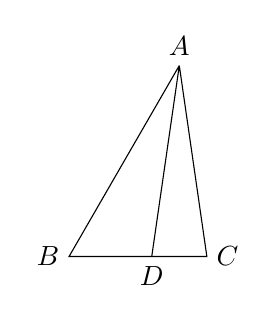
\begin{tikzpicture}[scale=0.35]
        \draw (4,6.928) coordinate (A) node[above] {$A$};
        \draw (0,0) coordinate (B) node[left] {$B$};
        \draw (5,0) coordinate (C) node[right] {$C$};
        \draw (3,0) coordinate (D) node[below] {$D$};
        \draw (A)--(B)--(C)--(A) (A)--(D);
    \end{tikzpicture}
    \caption{}\label{fig-180801-1830}
\end{minipage}
\end{figure}

\begin{exercise}
    如图~\ref{fig-180801-1830}, 在 $\triangle ABC$ 中, $B=\dfrac\pi3$, $AB=8$, 点 $D$ 在边 $BC$ 上,
    且 $CD=2$, $\cos\angle ADC= \dfrac17$.
    
    (1) 求 $\sin\angle BAD$;\qquad (2) 求 $BD$, $AC$ 的长.    
\end{exercise}
\beginsolution
    (1) 由题意, $\angle ADC= \angle B+ \angle BCD$, $\sin\angle ADC= \dfrac{4\sqrt3}7$, 所以
    \[\sin\angle BAD= \sin(\angle ADC- \angle B)
        = \dfrac{3\sqrt3}{14}.\]

    (2) 在 $\triangle ABD$ 中,
    \[\frac{BD}{\sin\angle BAD}= \frac{AB}{\angle ADB}
        = \frac{AB}{\angle ADC},\]
    所以 $BD=3$. 再考虑 $\triangle ABC$ 知,
    \[AC^2= BA^2+ BC^2- 2BA\cdot BC\cos B= 49,\]
    故 $AC=7$.
\endsolution